\section{Aufbau und Durchführung}
\subsection{Aufbau}
\begin{figure}
    \centering
    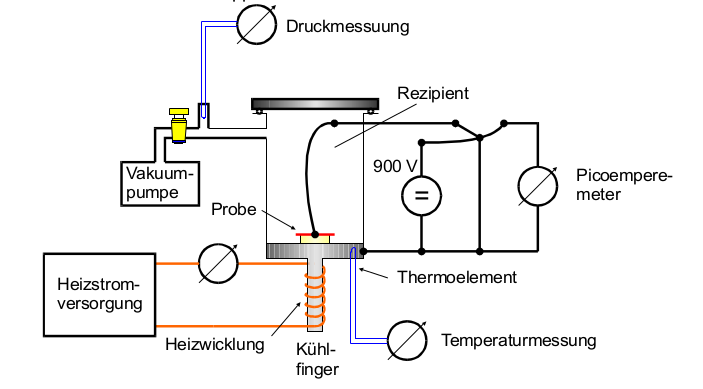
\includegraphics[width=0.8\textwidth]{bilder/Aufbau.png}
    \caption{"Schematischer Aufbau einer Anlage zur Messung der Dipolrelaxation.
            \cite{skript}}
    \label{fig:aufbau}
\end{figure}

Zentrales Element zur Messung ist die Probe selbst, die in den Rezipent gelegt wird. Diese gilt es im Verlauf entsprechend
zu erwärmen und zu kühlen. Als Probe lassen sich Kaliumbromid oder CsJ verwenden, die mit Strontium
dotiert sind. Die Aufwärmung erfolgt durch ein Heiznetzgerät, welches die Heitzarte durch Veränderung der angelegten Spannung ändern kann.
Hilfreich ist es diesen Prozess durch Wärmeleitpaste zu unterstützen um
Verlust durch nicht gut verbundene Kontaktflächen zu vermeiden.
Nötig ist es außerdem ein hinreichend gutes Vakuum in einem Reipenten von \SI{10}{\milli\bar} !!!10 hoch minus 2 eigetnlich, noch ändern !!!!! 
durch eine angeschlossene Vakuumpumpe zu erzeugen.
Eventuelle Druckmessungen  lassen sich durch ein Messgerät zwischen der Pumpe und dem Vakuum tätigen.
Oberhalb und unterhalb der Probe lässt es sich durch einen Plattenkondensator eine Spannung anlegen um so ein 
elektrisches Feld (um die Probe herum) zu erzeugen. Um die Temperatur zu messen bietet sich ein, am Aufbau angebrachtes, Thermometer an.
Kontrer zur Heißvorrichtung, lässt sie sich die Probe durch einen Kühlfinger, der in ein mit flüssigem Stickstoff gefülltes Dewar getaucht wird, 
abkühlen.
Ein empfindliches Picoampermeter, angeschlossen an den Kondensatorplatten, steht außerdem bereit im richitgen Moment auch kleine
Stromflüsse zu messen.

\begin{figure}
    \centering
    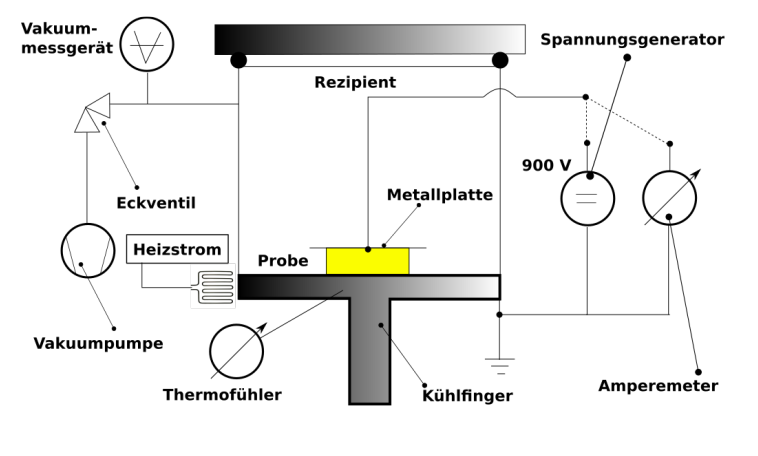
\includegraphics[width=0.8\textwidth]{bilder/aufbau2.png}
    \caption{"Schematischer Aufbau einer Anlage zur Messung der Dipolrelaxation mit 
            besonderem Fokus auf den Rezipten.
            \cite{skript}}
    \label{fig:aufbau2}
\end{figure}


Im Rezipenten selbst liegt auf der Probe noch eine Metallplatte um das elektrische Feld anlegen zukönnen.
Dieses Feld wir mit einer Spannung von bis zu $\SI{900}{\volt}$ aufrecht gehalten.
\\
\newline
\subsection{Durchführung}
Zunächst gilt es ein Vakuum im Rezipienten zu erzeugen. Dafür wird die Drehschieber-Vakuumpumpe
aktiviert die in der Lage ist einen Unterdruck von bis zu $\SI{10}{\milli\bar}$ !!!!hoch minus 2!!! aufrecht zu halten.
Dazu muss die Temperatur der Probe maßgeblich erhöt werden, auf bis zu $\SI{320}{\kelvin}$ für Kaliumbromit. Kontrolliert wird der Wert mit einem Thermometer.
Nun wird eine Spannung von $\SI{950}{\volt}$ an die Metallplatte, bzw. den Kondensator, angelegt. Es entsteht also ein elektrisches 
Feld durch die Probe hindurch. Der Kondensator braucht einige Zeit um vollständig geladen zu sein,
so soll also etwa $\SI{900}{\second}$ gewaret werden um eine hinreichende Ladung zu garantieren.
Außerdem ist die so gewählte Ladezeit groß gegenüber der Relaxationszeit $\tau$.
Sobald die Zeit abgelaufen ist, es bietet sich an diese mit einer Stoppuhr zu messen,
gilt es die Probe mit flüssigen Stickstoff auf etwa $\SI{210}{\kelvin}$ zu kühlen.
Bevor Messungen stattfinden dürfen, muss die elektrische Spannung ausgeschaltet werden.
Dadurch verschwindet auch das elektrische Feld der Probe. Da der Kondensator seine Ladung behalten wird,
muss dieser Kurzgeschlossen werden und es wird gewartet, bis dieser vollständig die von ihm erzeugte Spannung verloren hat.
Nach einigen Minuten darf das Picoampermeter angeschlossen werden. Jedoch muss,
wenn dies noch nicht der Fall ist, darauf gewartet werden bis der Stromwert konstant ist.
Mit der Heizstromversorgung soll die Probe nun wieder erwärmt werden, wobei die 
Heizrate, die konstant sein soll, gut beobachtet werden muss. Aus der thermodynamischen Natur 
folgt, dass es bei ansteigender Tempatur immmer mehr Arbeit braucht um etwaige Materie bei 
konstanter Umgebungstemperatur zu erwärmen. Also sei der Heizstrom variabel am Gerät
einstellbar und muss im Verlauf angepasst, bzw. erhöht werden.
\\
\newline
Die wichtigen Messdaten für den Versuch die es zu Messen gilt, ist die am Picoampermeter 
abgelesene Spannung beim Aufheizen und die dabei auftretende Temperatur der Probe.
Es werden zwei Messreihen gestartet, wobei die Heizrate von ursprünglich $\SI{2}{\degree\per\minute}$
auf $\SI{8}{\degree\per\minute}$ variiert wird.